\documentclass{article}
\setcounter{secnumdepth}{0}
\usepackage[utf8]{inputenc}
\usepackage{xcolor}
\usepackage{color}
\usepackage{caption}
\usepackage{enumitem}
\usepackage[colorlinks = true,
            linkcolor = blue,
            urlcolor  = blue,
            citecolor = blue,
            anchorcolor = blue]{hyperref}
\usepackage{hyperref, todonotes}



\title{Environment mapping with a mobile robot \\
\Large MSc thesis diary}
\author{Laszlo Debreczeni}
\date{March 2024 -- December 2024}
\graphicspath{ {./images/} }

\begin{document}
\maketitle

\tableofcontents
\newpage

\section{March 28 -- April 2}
\begin{itemize}
\item read about neural radiance fields \url{https://www.youtube.com/@thenerfguru}
\item read about 3D Gaussian Splatting \url{https://www.youtube.com/watch?v=VkIJbpdTujE}
\item try LumaAI \url{https://lumalabs.ai/} with iPhone RGBD
\item optionally try a 3D Gaussian Splatting reconstruction of your room (requires GPU) 
\end{itemize}
\newpage

\section{March 21 -- March 28}

\subsection{Tasks}
\begin{itemize}
\item Create own ROS2 workspace and create an own ROS2 node \url{https://docs.ros.org/en/foxy/Tutorials/Beginner-Client-Libraries/Creating-A-Workspace/Creating-A-Workspace.html} \todo[color=green!30]{DONE}
\item test SpectacularAI SDK \url{https://github.com/SpectacularAI/sdk-examples} \todo[color=blue!30]{IN PROGRESS}
\item VIO record, replay, visu \url{https://github.com/SpectacularAI/sdk-examples/tree/main/python/oak}
\item ROS wrapper: \url{https://github.com/SpectacularAI/sdk-examples/tree/main/python/oak/ros2}
\item Mapping ROS \url{https://github.com/SpectacularAI/sdk-examples/blob/main/python/oak/mapping_ros.py}

\item create a point cloud reconstruciton of your room
\url{https://www.youtube.com/watch?v=n34dt-Ag1Yo}
\end{itemize}

\subsection{Achievements}
\begin{itemize}
    \item Unfortunately, due to HDD crash and reinstall, the project is delayed by one week. The same tasks are valid for the next week. The solution was to buy a high speed, more reliable external HDD (ADATA HD650 in my case)
    \item A basic ROS2 workspace with packages containing nodes has been created \url{https://github.com/K0pasz/thesis_ros2_test_workspace}
    \item When I try out the SpectecularAI Python examples they log onto the terminal "SpectacularAI WARN: Dropping frames!
SpectacularAI WARN:   VIO may be running too slow, data is being input too fast, or IMU samples are missing / time-offset from frames. (buffer size 10)". SOLUTION: The problem was that the IMU's firmware version was too old. Had to update it, but the documentation is extremely poor about it. What I did: cloned \url{https://github.com/luxonis/depthai-python}, then ran \verb|python3 examples/install_requirements.py| and \verb|python3 examples/IMU/imu_firmware_update.py| which successfully updated the IMU's firmware.
    \item After the successful firmware update, I tried different Spectacular AI examples.
    \item IMU visualization:\par
    \begin{minipage}{\linewidth}
        \centering
        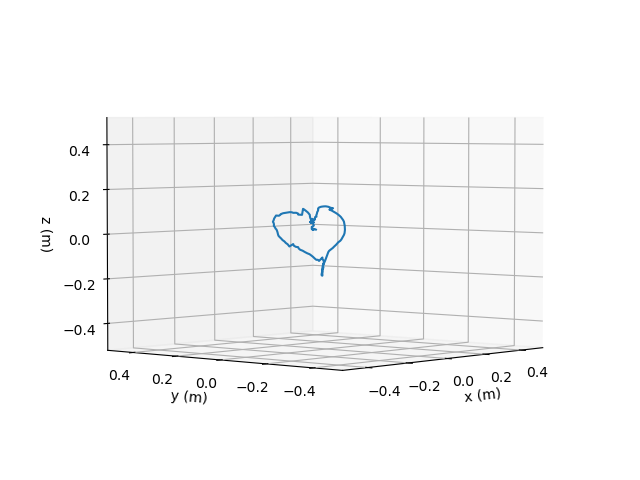
\includegraphics[width=1\linewidth]{spectacular_ai_vio_visu.png}
        \captionof{figure}{IMU visualization}
    \end{minipage}

    
\end{itemize}


\newpage

\section{March 12 -- March 19}

\subsection{What did I do}
\begin{itemize}
    \item DepthAI viewer:\par
    \begin{minipage}{\linewidth}
        \centering
        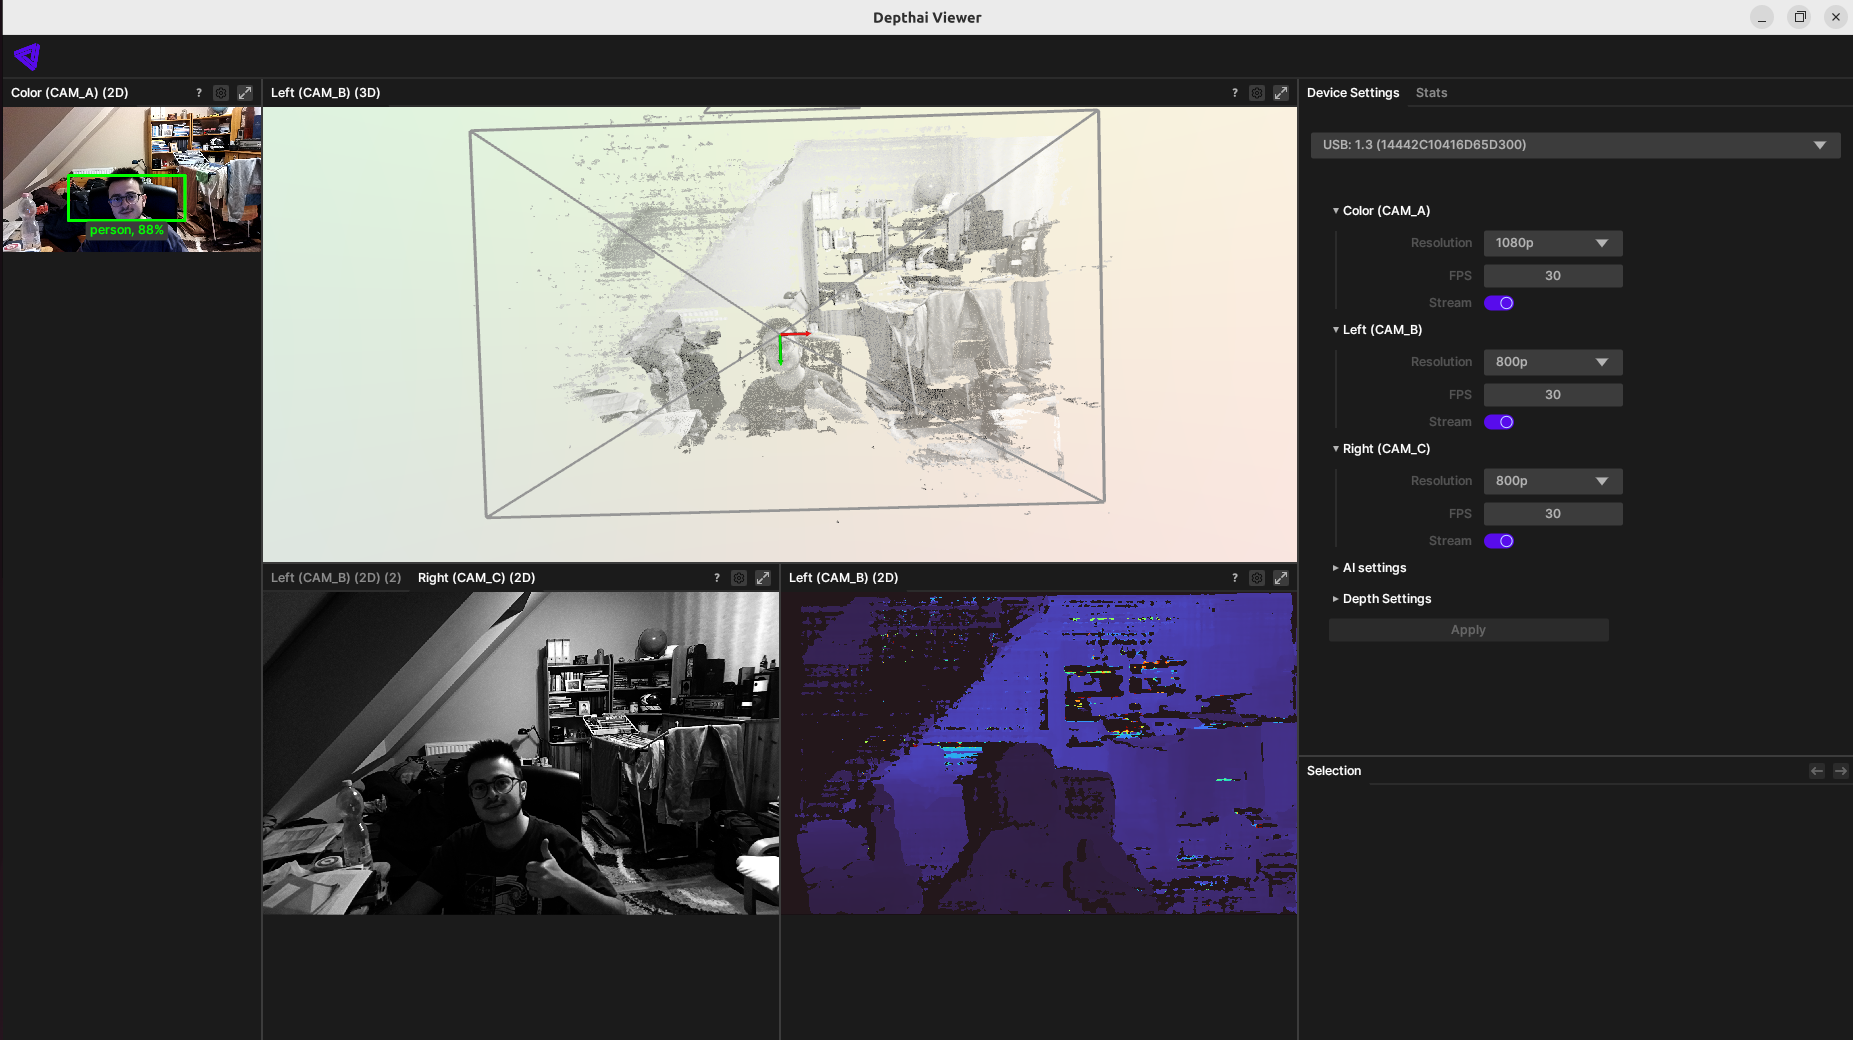
\includegraphics[width=1\linewidth]{depthai_viewer.png}
        \captionof{figure}{DepthAI Viewer}
    \end{minipage}
    \begin{minipage}{\linewidth}
        \centering
        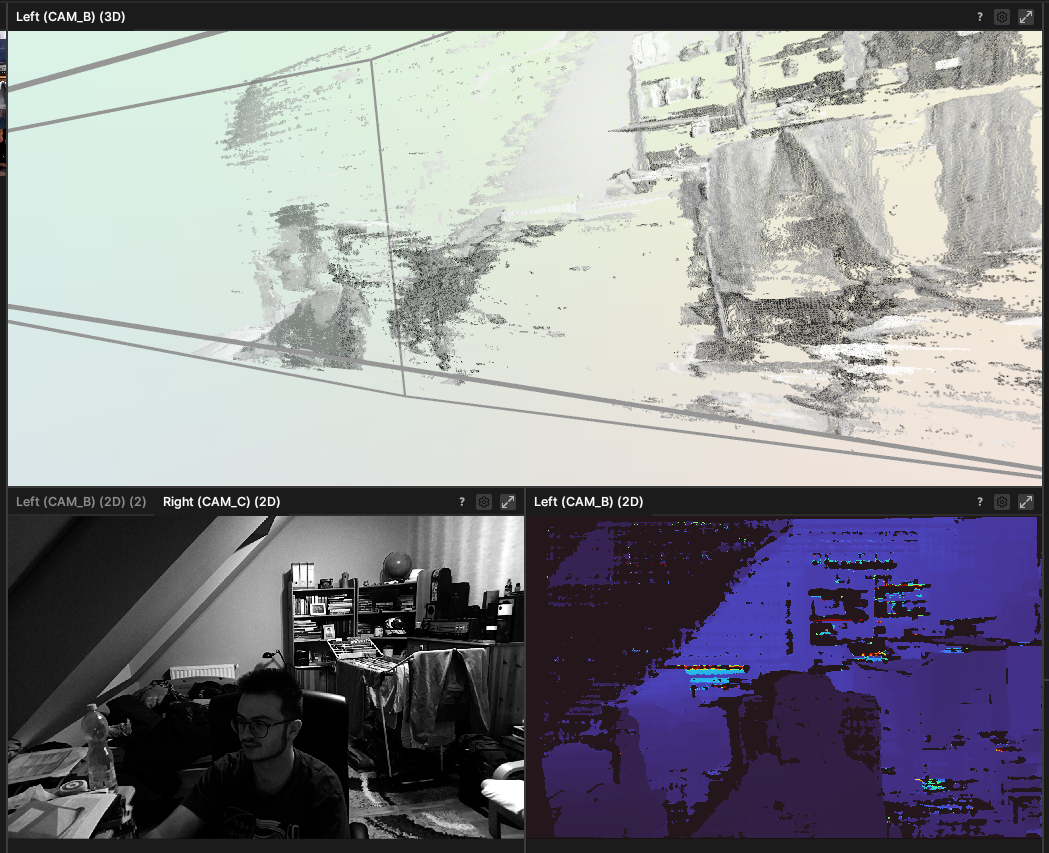
\includegraphics[width=1\linewidth]{depthai_viewer_3d.png}
        \captionof{figure}{DepthAI Viewer 3D reconstruction}
    \end{minipage}
    \item \url{https://docs.luxonis.com/en/latest/pages/slam_oak/}
    \item \url{https://github.com/SpectacularAI/sdk-examples/tree/main/python/oak}
        
\end{itemize}

\subsection{Reading}
Read about 
\begin{itemize}
    \item ORB\_SLAM (\url{https://github.com/raulmur/ORB_SLAM}) \todo[color=green!30]{DONE}
    \item ORB\_SLAM2 (\url{https://github.com/raulmur/ORB_SLAM2})\todo[color=green!30]{DONE}
    \item ORB\_SLAM3 (\url{https://github.com/UZ-SLAMLab/ORB_SLAM3}) \todo[color=green!30]{DONE}
    \item \url{https://webdiis.unizar.es/~raulmur/orbslam/} \todo[color=green!30]{DONE}
\end{itemize}


example citation \cite{Macenski2021}


\subsection{Links}
\begin{itemize}
\item ORB\_SLAM3 with OAKD Pro \url{https://github.com/duncanrhamill/oakd_orbslam3}
\end{itemize}

\subsection{Tasks}
\begin{itemize}
    \item Install the OAK-D camera's dependencies \todo[color=green!30]{DONE}
    \item Try out the DepthAI demos with the OAK-D camera \todo[color=green!30]{DONE}
\end{itemize}

\newpage

\section{March 5 -- March 12}
\begin{itemize}
    \item Turtlebot4 Lite offers maximum current of 1.9 A but Turtlebot4 (the more advanced one) offers only 300 mA \textrightarrow it's kind of weird
    \item Maybe static IP or self-evident hostname for the RPi?
    \item SpectecularAI could be used for large-scale mapping and real-time reconstruction of the area that is mapped with the camera
    \item This could be useful: \url{https://docs.luxonis.com/en/latest/pages/spatial-ai/}
    \item Using custom models on the OAKD: \url{https://docs.luxonis.com/en/latest/pages/model_conversion/}
    \item Running a model on low performance devices (such as the RPi on the Turtlebot4): \url{https://docs.luxonis.com/en/latest/pages/tutorials/local_convert_openvino/}
    \item Camera depth map to point cloud: \url{https://docs.luxonis.com/en/latest/pages/tutorials/device-pointcloud/}
\end{itemize}

\subsection{Reading}
\begin{itemize}
\item read about Turtlebot4 \url{https://turtlebot.github.io/turtlebot4-user-manual/}\todo[color=green!30]{DONE}

\item read about ROSBot2 \url{https://husarion.com/manuals/rosbot/}\todo[color=green!30]{DONE}

\item read about Spectacular AI \url{https://spectacular.ai/}\todo[color=green!30]{DONE}

\item read about DepthAI/OAKD\todo[color=green!30]{DONE}
\begin{itemize}
    \item \url{https://docs.luxonis.com/en/latest/pages/tutorials/first_steps/}
    \item  \url{https://shop.luxonis.com/collections/product-guide}
\end{itemize}

\item read about ROS2 \url{https://github.com/ros2/ros2}\todo[color=blue!30]{IN PROGRESS}


\end{itemize}


\subsection{Tasks}
\begin{itemize}
    \item Install Ubuntu 22\todo[color=green!30]{DONE}
    \item Install ROS2 Humble \url{http://docs.ros.org/en/humble/}\todo[color=green!30]{DONE}
    \item Basic ROS2 tutorials \url{http://docs.ros.org/en/humble/Tutorials.html}\todo[color=blue!30]{IN PROGRESS}
    \item Try out \url{https://turtlebot.github.io/turtlebot4-user-manual/software/turtlebot4_simulator.html}
    \item Try out \url{https://turtlebot.github.io/turtlebot4-user-manual/software/rviz.html}
    \item Try out \url{https://turtlebot.github.io/turtlebot4-user-manual/software/simulation.html}
    \item Try out on the robot: \url{https://turtlebot.github.io/turtlebot4-user-manual/tutorials/}
\end{itemize}

\newpage


\iffalse
\section{EXAMPLE SECTION March 4 -- March 10}
\line(1,0){\linewidth}

\subsection{Current Hurdle/Problem}
\begin{itemize}
\item 
\end{itemize}
\subsection{Reading}
\begin{itemize}
\item 
\end{itemize}

\subsection{Programming}
\begin{itemize}
\item 
\end{itemize}
\subsection{Writing}
\begin{itemize}
\item 
\end{itemize}
\subsection{Insights Gained On the Current Problem}
\begin{itemize}
\item 
\end{itemize}
\subsection{Any Inspiration?}
\begin{itemize}
\item 
\end{itemize}
\subsection{Questions}
\begin{itemize}
\item 
\end{itemize}
\subsection{What's next?}
\begin{itemize}
\item
\end{itemize}
\newpage
\fi

\section{Highlighting Overview}

\colorbox{green}{Successfully completed}\\
\colorbox{yellow}{Pending}\\
\colorbox{orange}{Successfully completed, but didn't solve the problem/but has not effect on the process of the project.}\\
\colorbox{red}{Failed/Not Working}\\
\newpage



\bibliographystyle{plain}
\bibliography{main}

\end{document}
